\documentclass[11pt,a4paper,oneside,notitlepage]{report}
\usepackage[english]{babel}

\setlength{\hoffset}{-1in}
\setlength{\voffset}{-1in}
\setlength{\topmargin}{2cm}
\setlength{\headheight}{0.5cm}
\setlength{\headsep}{1cm}
\setlength{\oddsidemargin}{2.5cm}
\setlength{\evensidemargin}{2.5cm}
\setlength{\textwidth}{17cm}
\setlength{\textheight}{23.3cm}
\setlength{\footskip}{1.5cm}

\usepackage{titlesec}
\usepackage{fancyhdr}
\usepackage{graphicx}
% \usepackage[colorlinks]{hyperref}

%\pagestyle{fancy}
\titleformat{\chapter}{}{}{0em}{\bf\LARGE}
\renewcommand{\chaptermark}[1]{\markright{\MakeUppercase{#1}}}
\renewcommand{\sectionmark}[1]{\markright{\thesection~#1}}
\titlespacing*{\chapter}{0pt}{-40pt}{10pt}

\newcommand{\headerfmt}[1]{\textsl{\textsf{#1}}}
\newcommand{\headerfmtpage}[1]{\textsf{#1}}

\fancyhf{}
\fancyhead[LE,RO]{\headerfmtpage{\thepage}}
\fancyhead[LO]{\headerfmt{\rightmark}}
\fancyhead[RE]{\headerfmt{\leftmark}}
\renewcommand{\headrulewidth}{0.5pt}
\renewcommand{\footrulewidth}{0pt}

\fancypagestyle{plain}{ % eerste bladzijde van een hoofdstuk
  \fancyhf{}
  \fancyhead[LE,RO]{\headerfmtpage{\thepage}}
  \fancyhead[LO]{\headerfmt{\rightmark}}
  \fancyhead[RE]{\headerfmt{\leftmark}}
  \renewcommand{\headrulewidth}{0.5pt}
  \renewcommand{\footrulewidth}{0pt}
}

\renewcommand{\baselinestretch}{1.5}
\hyphenation{ditmagnooitgesplitstworden dit-woord-splitst-hier}

\begin{document}

% title
%  Titelblad

% Opmerking: gaat uit van een \baselinestretch waarde van 1.5 (die moet
% ingesteld worden voor het begin van de document environment)

\begin{titlepage}

\setlength{\hoffset}{-1.3in}
\setlength{\voffset}{-1in}
\setlength{\topmargin}{1.5cm}
\setlength{\headheight}{0.5cm}
\setlength{\headsep}{1cm}
\setlength{\oddsidemargin}{3cm}
\setlength{\evensidemargin}{3cm}
\setlength{\footskip}{1.5cm}
\enlargethispage{1cm}
% \textwidth en \textheight hier aanpassen blijkt niet te werken

\fontsize{14pt}{16pt}
\selectfont

\begin{center}


\includegraphics[height=2cm]{fig/ruglogo}

\vspace{0.5cm}

Faculty of Engineering and Architecture\\
Computer Science Engineering\\

\vspace{3.5cm}

\fontseries{bx}
\fontsize{19.28pt}{23pt}
\selectfont

Advanced Multimedia Applications\\ 
Apps4Ghent\\
Progress Report

\fontseries{m}
\fontsize{14pt}{16pt}
\selectfont

\vspace{2.2cm}

Jeroen ARENS\\
Enver BRAL\\
Harald DE BONDT\\
Damian TARNACKI


\vspace{6.4cm}

Academic year 2014--2015

\end{center}
\end{titlepage}

% geen paginanummering tot we aan de inhoudsopgave komen
\pagestyle{empty}

% table of contents
\tableofcontents

\chapter{Introduction}

The library of Ghent has a massive considerable amount of data regarding its collection of books and the people it lends books to. The library is considering to provide this data source as open data that is accessible by everyone. The purpose of this project is to think of and develop a creative tool/app/website that uses this open data, which will be used in the library of Ghent itself and will also be used to promote the university of Ghent as a multimedia university. The project is executed in regard of the AppsForGhent edition of 2015, which tries to stimulate the use of open data and the development of applications that use the data which has been put publicly accessible.\\
\\
Besides this project, we need to provide a REST API so that other developers can use the library data by using our API. Also a second application will be made, with the REC as demanding party to provide the most lent books during the summer vacation, when looking to the age and the sex of a person.\\
\\
To accomplish this project, a multi-disciplinary team will be assembled consisting of students of engineering, communication science, data analysts and economists. Together a well-thought and good looking/functioning concept will be rolled out.

\chapter{General project decisions}

\section{Role decisions}

\begin{itemize}
 \item Jeroen will execute the role of Project Leader. He will take care of the communication between the client and the different groups of students. (13/02)
 \item Jeroen will be the scheduler for this project. (25/02)
 \item Harald will be the continuous integration manager. (25/02)
 \item Damian will take care of the tasks of the system administrator. (25/02)
 \item Damian will take care of continuous integration system. (3/03)
 \item Harald will be reponsible for frontend matters. (3/03)
 \item Enver will focus on providing API. (3/03)
 \item Jeroen will help with Django related problems in backend due to his experience. (3/03)
\end{itemize}

\section{Infrastructure decisions}
\begin{itemize}
	\item A private git repository is set up via Github on which the project development will take place.
    \item To keep the communication clear and well structured, Slack is used to handle the communication between the computer science students. Communication with other sources will be done by email.
    \item Slack will also be used for stand-up meetings with the group. If a call is needed, Google hangouts (integrated into Slack) will be used.
\end{itemize}

\section{Risks}

\begin{center}
  \begin{tabular}{ l | c | r  }
    \hline
    Risk & Level & Impact \\ \hline
   & & No interesting website for the library\\
      Frontend is not interactive & H & . Also no story can be extracted\\
    & &  for the journalist students \\
    Data not specific enough & M & Features can be less accurate \\
    Data not available on time & M & Less features can be constructed\\
  \end{tabular}
\end{center}

\section{Technologies used}

\begin{itemize}
	\item Django with django REST framework for the web application and API.
	\item Apache2 webserver with Web Server Gateway Interface (WSGI) for serving Python applications.
	\item MongoDB No-SQL database to store JSON-like documents, consistent with JSON-LD mapping.
  \item HighCharts and HighMaps for visualisation on the client side.
  \item RML for mapping CSV data to JSON-LD
\end{itemize}

Open source licences and fast development for all above components outweighed usage of other technologies.



\chapter{Application}
\section{Architecture}
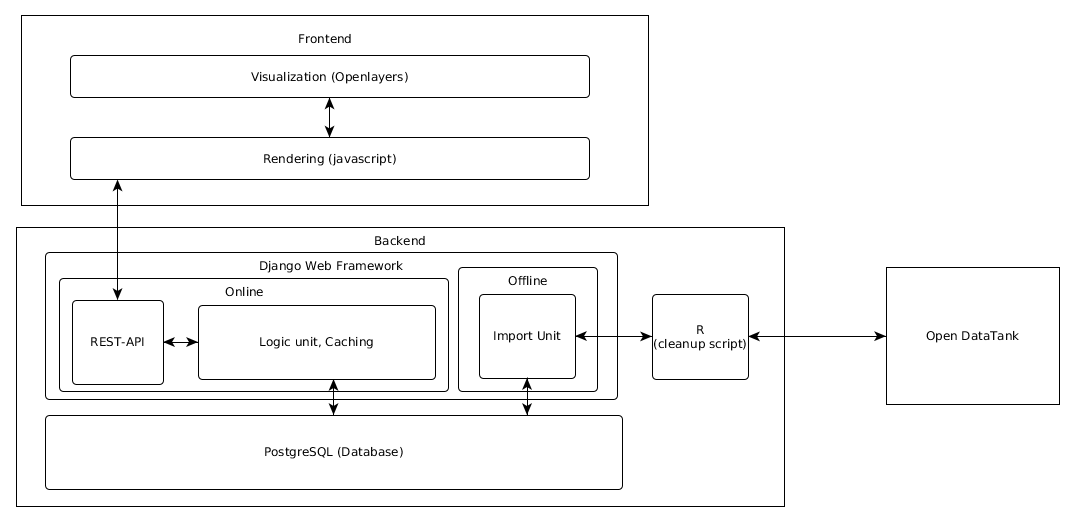
\includegraphics[width=16cm]{fig/Architecture}

\subsection{Frontend}
At the frontend side of our web application, we will have two main components, a rendering component and a visualization component. At the rendering block, the data requested via the API from the backend will be transformed into e.g. figures, dots, that can be displayed on the browser. When the transformation is finished, the visualization block will show the transformed data on the website itself.

\subsection{Backend}
We make use of 3 main components in the backend. First there is the RML unit which will be used to make a mapping between the data of the Open Datatank towards a Linked Data JSON format. The second component is the database, for which we will use MongoDB so we can create a semantical database. As last main component, we have the django web framework. The blocks in this framework consist of an online and offline section. In the online section we have the REST-API which will be used to open up our data to our website and also towards other applications because of the open data concept. Besides this REST-API there is also a logical unit where the caching of requests, data,... will happen. At the offline section of the Django Web Framework, we will provide an import unit to put the JSON-LD data into the database. This is an offline block since the data is provided as a data dump and only needs to imported once. Since it will make use of the mapping that Django provides between the database and Python objects, it is included in the Django block.

\section{Functional requirements}

\subsection{User interface}

On initial load of the webpage an empty map of Ghent is shown with one big number counting the sum of all books ever loaned. This map is divided in statistical sectors. The shape of these sectors is dynamic (online available) and will be retrieved every time the page is loaded. Under the map will be a slider showing the time span for the data published. Every sector can be selected, if none is, the data represented is for all of Ghent.  The numbers shown are the amount of books that fit the query. The query is defined by the optional arguments; sector, time span and properties of the books. An example; sector="A2", book: genre="horror". This query will give the amount of horror books loaned in sector A2 from the oldest (1996) to the youngest (2014) data (because time span is not specified). The book properties of the query are given in an input section above the map. Also shown on the map are distribution locations (libraries). A second layer of visualised data shows where books are loaned from. This relation between statistical sector and library can be visualised by a line. The user can zoom in and out on this map and it's visualised data by scrolling.

\subsection{API}

In order to provide data to the frontend and external services (such as linked data applications), an API has to be decided on. The aim of this section is to give an overview of the calls that can be made this API and the kind of data it will return.

\subsubsection{Root URL}

{\bf Usage}:
\begin{verbatim}
http://api.honegger.elis.ugent.be/v1/}
\end{verbatim}

The API will be accessible through URLs that start with \texttt{http://api.honegger.elis.ugent.be/v1/}, where \texttt{v1} indicates the major version of the API. This version number is included so future versions of the API can deprecate certain parts without having to worry about external services breaking because of these changes.

\subsubsection{Items}

{\bf Usage}:
\begin{verbatim}
http://api.honegger.elis.ugent.be/v1/items/[?param_1=value_1]
  [&param_2=value_2]...[&param_n=value_n][/count]
\end{verbatim}

{\bf Parameters}:
\begin{itemize}
  \item \texttt{sector}: Identifier for the statistical sector. When provided, only items that were loaned by people living in the given sector will be returned.
  \item \texttt{age\_description}: Description of the target age of the item.
  \item \texttt{from\_date}: When provided, only items that were loaned after (and including) the given date are returned.
  \item \texttt{until\_date}: When provided, only items that were loaned before (and including) the given date are returned.
  \item \texttt{limit}: The maximum number of items that should be returned.
  \item \texttt{order}: A comma-seperated list of properties on which to sort the data in ascending order. Descending order can be achieved by adding a $-$ before the property.
\end{itemize}

The main resources that are provided by the API are \emph{items} present in the library, such as \emph{books} and \emph{DVDs}.
By calling the URL listed above, a list of \emph{items} can be fetched that can be filtered using various optional parameters.
The return value should be a list of \emph{items} containing their unique identifiers, various metadata properties (such as title, genre, theme, ...), the library the item was loaned from and the number of times the items was loaned, given the parameters.\\

Because the main visualisation can get away with only the number of loans for all items given a set of parameters, an extra \texttt{/count} action can be used, which simply returns the number of loans instead of a list of items.

\section{Use case}

The library personel can use the web application in two ways, reactively and pro-actively. Respectively by searching on a specific book (title) or on a certain group of books (genre, target-age,...) and look for differences between current distribution (visualised per library) and preffered distribution (visualised per sector). If the demand of a certain book is skewed for a sector, the copies can be moved closer (closer library) to this sector. If the demand of a group correlates with a sector the personel can decide to anticipate the demand of similar books in this group and move the whole group.


\chapter{Overview of meetings}

\section{Meeting with Team 13/02}
{\bf present}: Everyone of the team\\
{\bf purpose}: Assign team leader who will contact the client to schedule a meeting.\\
{\bf result}: Jeroen is assigned as team leader, he will make an appointment with our client during the 3rd week of the semester.

\section{Meeting with Client 25/02}

{\bf present}: Everyone of the team, Professor Mannens, Koen from Digipolis, Professor Van den Poel, Pieter Colpaert from REC, Pieter Blomme, 2 spokes people from the library and Leenke (journalist student)\\
{\bf purpose}: First introduction to every party and getting to know the scope of the project.\\
{\bf result}:
\begin{itemize}
\item Each party discussed their involvement in the project and what they would like to gain from it. This information will be used to define the actual output of the project. We proposed a website that visualizes borrowed books on a map of Ghent. All parties agreed this would (in some way) fit in with their individual goals.
\item The library of Ghent has two goals in mind. The first one is to make the distribution of books between the different libraries at Ghent more efficient. The idea is to find correlations based on geographical data to predict what kind of books need to be available at the different library sites.\\ The second suggestion is to define new (hidden) genres. These can be used to recommend books towards the readers themselves.
\item The journalists want to find a story which can be interesting for the people of Ghent. This needs to be presented in a creative manner.
\item The master students of marketing want to use the data to do analysis upon. Based on this analysis, they can develop a predictive model in regard with the books and users at the library.
\item REC wants to have an inspiring project and wants to profile the UGent as a multimedia university.
\item A lot of suggestions were given at the meeting and have been documented in a separate document so that they may be used to figure out what can be done within the limited time that is provided to us, as well as to give us inspiration for future suggestions.
\end{itemize}
\section{Meeting with Team 25/02}
{\bf present}: Everyone of the team\\
{\bf purpose}: Define an initial scope to work upon during the semester
\begin{itemize}
\item For the front-end of the website, first a user interface will be developed on which queries can be executed by the journalists as aid for them to find a story behind the data. Afterwards the visualization of this data will be made more creative. E.g. an interactive map with the data displayed, several graphs, ...
\item To store the data at the back-end a NoSQL database tool will be used. The tool we will use is MongoDB. With MongoDB we can store the data and already make a basis semantical network. For the data-analysis, a basic model can be employed which will just look at obvious correlations. Later on the students of marketing can analyse the data to enhance this model.
\end{itemize}

\section{Meeting with Prof. Mannens 26/02}
{\bf present}: Prof Mannens, assistent, everyone of the team\\
{\bf purpose}: Discuss previous meetings and decide on what needs to be done next, get some feedback about the current progress and our current approach\\
\begin{itemize}
  \item We should focus our attention on the two most important clients, being the library of Ghent and the city of Ghent. We should then try to find a way to incorporate the journalists students into the project.
  \item Just forget about the marketing students, since we can't satisfy their needs.
  \item We will focus on using \textbf{open data} instead of the raw data.
  \item The most promising project we will focus on is a \emph{visualisation of the distribution of the books across Ghent over time}.
  \item If possible it might be nice to incorporate the concept of \emph{Goodreads}, which we could suggest on the \emph{data dive}.
\end{itemize}

\section{Meeting with Team 26/02}
{\bf present}: Everyone of the team\\
{\bf purpose}: Discuss feedback, decide on architecture\\
\begin{itemize}
  \item We worked out the basic of the architecture and identified the biggest separate blocks as \emph{Fronted}, \emph{Backend}, \emph{Database} and \emph{Syncing}.
  \item We decided to use Django on the backend.
  \item On the frontend (obviously) HTML5/CSS/Javascript will be used. A visualisation framework for drawing maps and charts still needs to be discussed before the next meeting with the client.
  \item The syncing part will be written in Python to minimise the number of different languages used and can probably be integrated into Django.
  \item A REST API will need to be decided to provide communication between frontend and backend.
  \item As soon as the data for the library is put online, we can start defining the Rest API between the \emph{Syncing} block and the \emph{TheDataTank} endpoint.
\end{itemize}

\section{Meeting with journalists 03/03}
{\bf present}: Pieter Blomme, Pieter Colpaert, both journalist students, everyone of the team\\
{\bf purpose}: Discuss what we decided on and what the journalists want from us\\
\begin{itemize}
  \item We explained what was discussed during our meeting with prof. Mannens and told them the project we decided on and its scope.
  \item The journalists need to find a story using our visualisation. They will present their ideas to Pieter Blomme, who will then help to select the final story by the main AppsforGhent event on 21/03.
  \item Leenke would like to be involved in every aspect of the project. As such, she would like to be notified of any meetings concerning the technical parts of the project and, when possible, attend them.
  \item We asked Pieter Colpaert for a server on which we could host the application, which he would provide as soon as possible.
  \item Damian will setup a sample Django project with MongoDB in a production environment, as soon as we have access to the server.
  \item Harald will focus on the frontend. Highcharts was suggested for drawing charts and maps and he will look into the usability of the framework or come up with a better alternative.
  \item Enver will work on the syncing between data provided by \emph{TheDataTank} and \emph{MongoDB}. He will also work on the REST API provided to the frontend by the backend.
  \item Jeroen will focus on the backend and will help out with all problems that are Django related (including setting up the production and development environments).
\end{itemize}

\section{Short meeting with people from the library 03/03}
{\bf present}: Pieter Blomme, Leenke Dedonder, everyone of the team, person from the library\\
{\bf purpose}: Give an update on what decided and inform the library on the next steps\\
\begin{itemize}
  \item We explained the scope of the project and afterwards we decided that the scope fits into what they would like to gain from this project.
\end{itemize}

\section{Short meeting about linked data 09/03}
{\bf present}: Pieter Colpaert, Anastasia Dimou, Leenke Dedonder, everyone of the team\\
{\bf purpose}: Inform us about a project Pieter's team will be working on for AppsForGent.
\begin{itemize}
  \item Pieter informed that a team would be working on a project that involves linked data. As a first step they would need to transform the library data (provided as CSV) to linked data.
  \item They would like it if we could make our data available as linked data as well, as such we have decided on using the same mapping from CSV to JSON-LD.
  \item We will also need to provide an API that returns JSON-LD data.
\end{itemize}

\chapter{Overview of events}
\section{Apps for Ghent data-dive 09/03}
{\bf present}: Pieter Colpaert, Leenke Dedonder, Everyone of the team except Damian\\
{\bf purpose}: Attend presentations about open data that is provided/available concering the libraries of Ghent and their collections\\
{\bf results}:
\begin{itemize}
  \item It became clear that the data that is provided to us lacks a lot of metadata about the books (e.g: authors, genre, number of pages, ...), but does provide general identifiers that could be used to hook into other services (e.g. ISBN).
  \item The Bibnet catalogus API could be used to get the additional metadata that is lacking from the library data set.
  \item A lot of data on the collection of books in the UGent are also provided as open data and appears to be uniquely identified by URLs. This might be useful in the context of linked data.
\end{itemize}

\section{Apps for Ghent Competition 21/03}
{\bf present}: Pieter Colpaert, Pieter Blomme, Journalism students, Everyone of the team\\
{\bf purpose}: Roll out our concept to convince the jury of our plan on the hackaton of Apps for Ghent\\
{\bf results}: 
\begin{itemize}
  \item The data that was provided by the library of Ghent was difficult/impossible to process during the hackaton. A concept was thus rolled out, but the implementation was not yet present. It is maybe better to work with the Bibnet API to get the data
  \item Another concept was invented by the journalism students and Pieter Blomme, where a recommendation system is build for summer books to take on vacation. Also a measure of how many books you can take with you will be shown. It is not yet sure if we should pursue this idea or rather stick to the plan using the geolocation data of the library. There is already a mockup of the concept, what was done on the hackaton.
  \item There was another team at the apps for ghent competition who managed to create the visualization of the library data at the hackaton. They are willing to send us the cleaned up data and the code/ info about the tools they used with which they managed to complete the task. This can give a boost to our project.
  \item At the end of the competition, we managed to get one of the prices, the price of Nerdlab, and also an honorable mention of the jury.
\end{itemize}

%dit moet nog binnen dutch komen, anders staat er Bibliography
\begin{thebibliography}{99}

%referenties zijn typisch in het Engels
\selectlanguage{english}
 
\bibitem{leos2000} K. Steenbergen, F. Janssen, J. Wellen, R. Smets, T.
Koonen,
\newblock ``Fast wavelength-and-time slot routing in hybrid fiber-access
networks for IP-based services'',
\newblock in {\em IEEE LEOS Symposium}, Delft, The Netherlands,
October~2000.
 
\bibitem{2-BIT} K. Nichols, V. Jacobson, L. Zhang,
\newblock ``A two-bit differentiated services architecture for the
Internet'',
\newblock {\em IETF RFC~2638},
July~1999.                                       

\bibitem{omniorb} http://www.omniorb.org

\end{thebibliography}

\selectlanguage{english}

%start



\end{document}
